\documentclass[tikz,border=8pt]{standalone}
% Shared preamble for the bootqcc TikZ figures.
\usepackage[T1]{fontenc}
\usepackage{helvet}
\renewcommand{\familydefault}{\sfdefault}
\usepackage{amsmath}
\usetikzlibrary{arrows.meta,positioning,shapes.geometric,fit,backgrounds,calc}

\definecolor{navy}{HTML}{1F3A5F}
\definecolor{sky}{HTML}{5AA9E6}
\definecolor{coral}{HTML}{FF6B6B}
\definecolor{slate}{HTML}{6B7A8F}

\tikzset{
  box/.style={rectangle, rounded corners=4pt, draw=navy, fill=sky!15, thick,
              align=center, minimum height=1.0cm, inner sep=6pt, text width=4.6cm},
  inbox/.style={rectangle, rounded corners=4pt, draw=slate, fill=slate!10, thick,
              align=center, minimum height=0.9cm, inner sep=5pt, text width=3.0cm,
              font=\small},
  io/.style={trapezium, trapezium left angle=72, trapezium right angle=108,
             draw=navy, fill=white, thick, align=center, minimum height=1.2cm,
             inner sep=5pt, text width=3.0cm},
  result/.style={rectangle, rounded corners=8pt, draw=coral, fill=coral!10, thick,
              align=center, minimum height=1.0cm, inner sep=6pt, text width=4.0cm},
  term/.style={rectangle, rounded corners=12pt, draw=navy, fill=navy, text=white,
               thick, align=center, minimum height=0.9cm, inner sep=6pt, text width=4.2cm},
  dec/.style={diamond, aspect=2.6, draw=navy, fill=white, thick, align=center,
              inner sep=0pt, text width=2.7cm, font=\small},
  err/.style={rectangle, rounded corners=4pt, draw=coral, fill=coral!15, thick,
              align=center, minimum height=0.9cm, inner sep=6pt, text width=3.2cm},
  arr/.style={-{Latex[length=3mm]}, thick, navy},
  lab/.style={font=\footnotesize\bfseries, text=navy, fill=white, inner sep=1.5pt},
  phase/.style={rounded corners=8pt, draw=navy!45, dashed, thick, inner sep=12pt},
}

\begin{document}
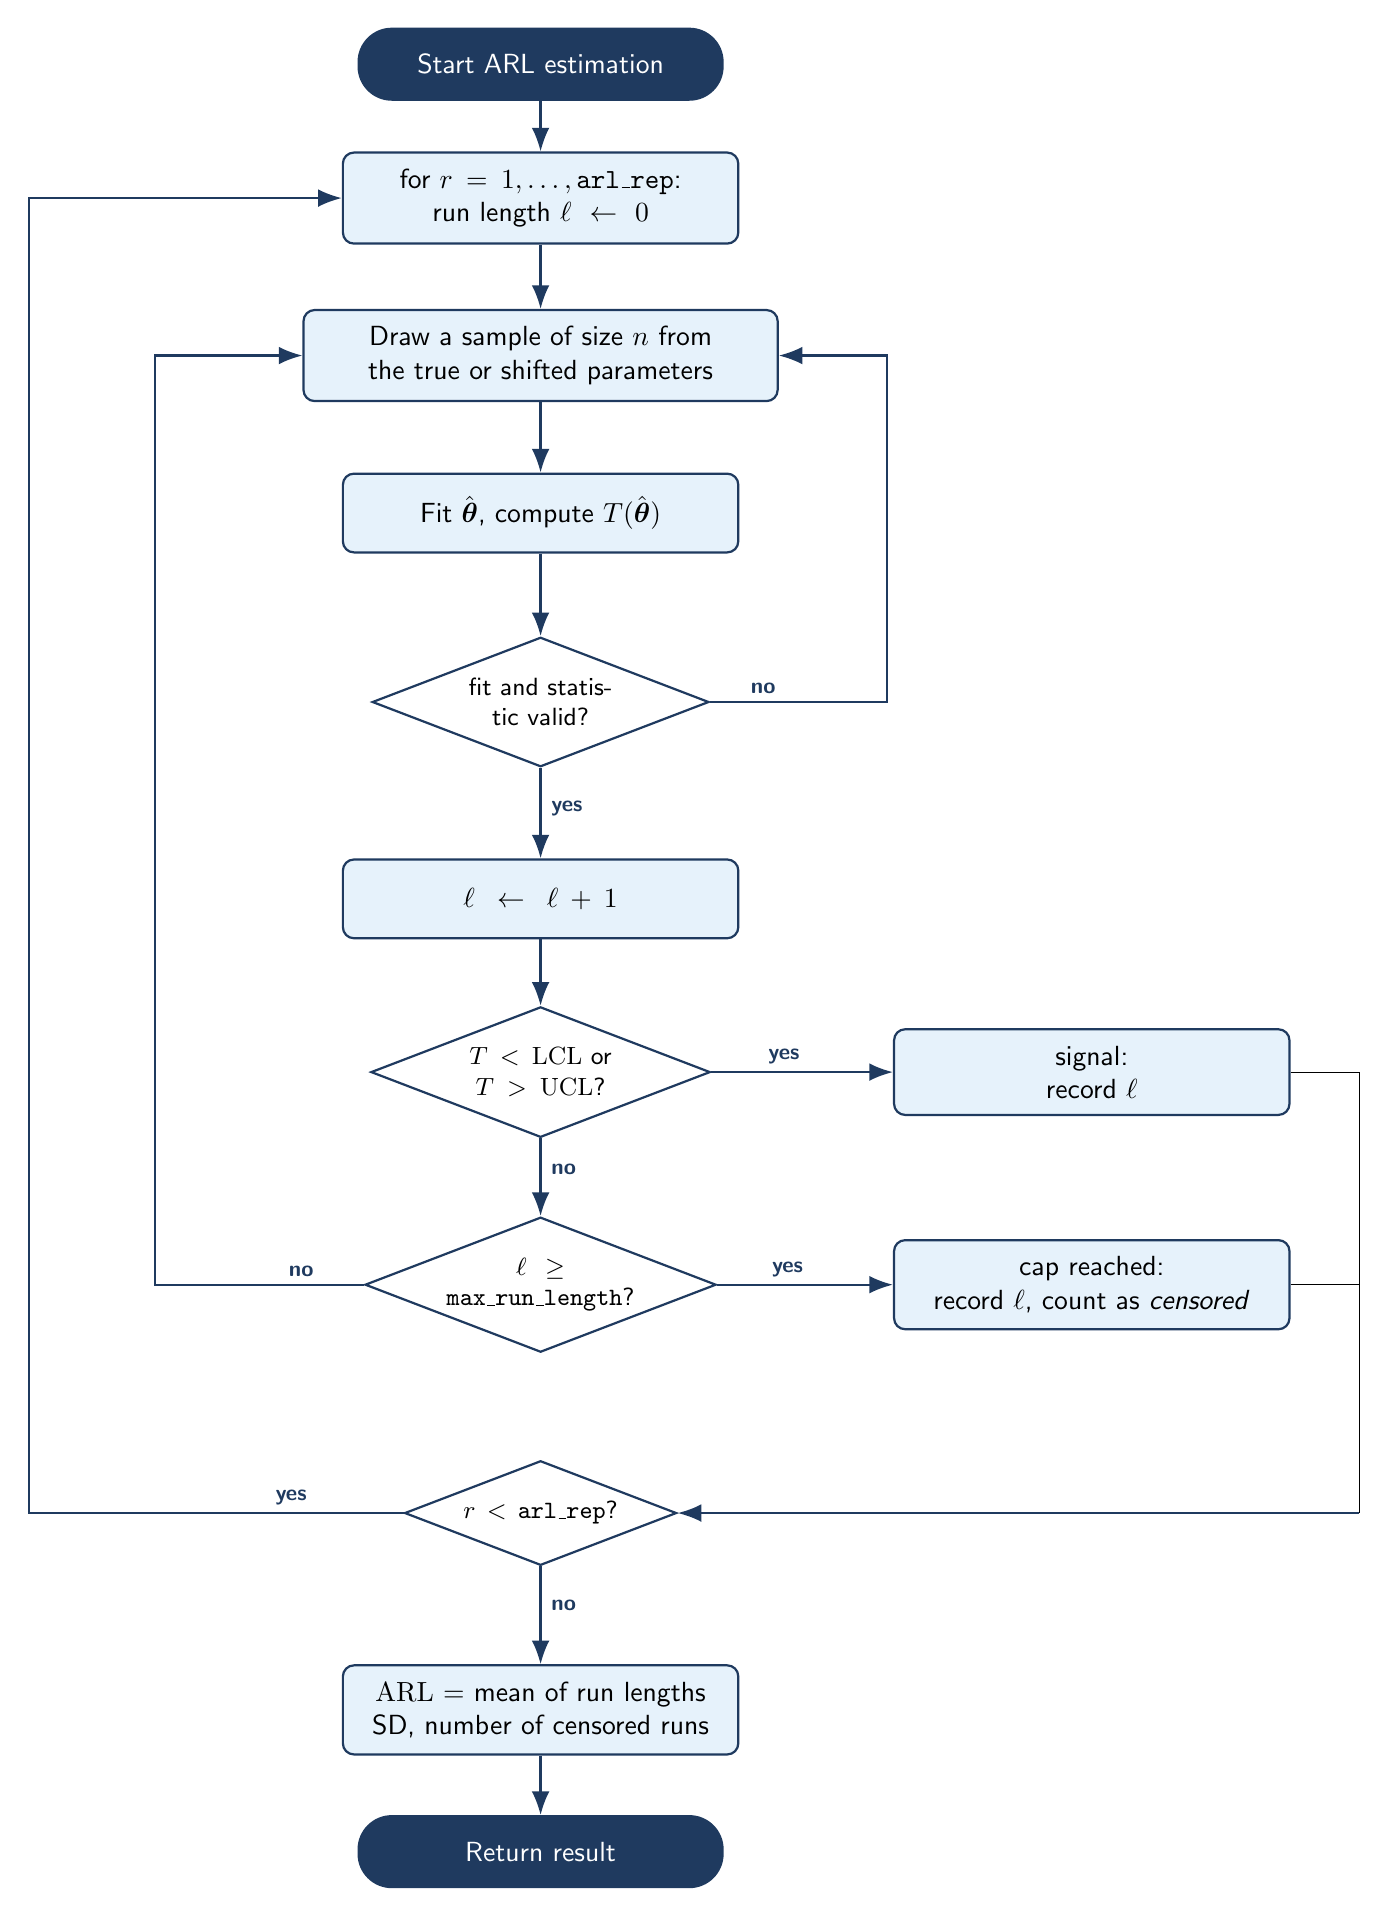
\begin{tikzpicture}

  \node[term] (start) at (0,0) {Start ARL estimation};
  \node[box]  (init)  at (0,-1.7)
    {for $r=1,\dots,\texttt{arl\_rep}$:\\ run length $\ell\leftarrow 0$};
  \node[box, text width=5.6cm]  (draw)  at (0,-3.7)
    {Draw a sample of size $n$ from\\ the true or shifted parameters};
  \node[box]  (fit)   at (0,-5.7)
    {Fit $\hat{\boldsymbol\theta}$, compute $T(\hat{\boldsymbol\theta})$};
  \node[dec]  (valid) at (0,-8.1) {fit and statistic valid?};
  \node[box]  (incr)  at (0,-10.6) {$\ell\leftarrow\ell+1$};
  \node[dec]  (out)   at (0,-12.8) {$T<\mathrm{LCL}$ or $T>\mathrm{UCL}$?};
  \node[dec]  (cap)   at (0,-15.5) {$\ell\ge$ \texttt{max\_run\_length}?};

  \node[box]  (rec1)  at (7.0,-12.8) {signal:\\ record $\ell$};
  \node[box]  (rec2)  at (7.0,-15.5) {cap reached:\\ record $\ell$, count as \emph{censored}};

  \node[dec]  (rdec)  at (0,-18.4) {$r<\texttt{arl\_rep}$?};
  \node[box]  (res)   at (0,-20.9)
    {$\mathrm{ARL}$ = mean of run lengths\\ SD, number of censored runs};
  \node[term] (end)   at (0,-22.7) {Return result};

  \draw[arr] (start) -- (init);
  \draw[arr] (init)  -- (draw);
  \draw[arr] (draw)  -- (fit);
  \draw[arr] (fit)   -- (valid);
  \draw[arr] (valid) -- node[lab, pos=0.45, right=2pt] {yes} (incr);
  \draw[arr] (incr)  -- (out);
  \draw[arr] (out)   -- node[lab, pos=0.4, right=2pt] {no} (cap);
  \draw[arr] (out)   -- node[lab, pos=0.4, above=1pt] {yes} (rec1);
  \draw[arr] (cap)   -- node[lab, pos=0.4, above=1pt] {yes} (rec2);
  \draw[arr] (rdec)  -- node[lab, pos=0.4, right=2pt] {no} (res);
  \draw[arr] (res)   -- (end);

  % failed fit: the run length is not increased, redraw
  \draw[arr] (valid.east) -- node[lab, pos=0.3, above=1pt] {no} (4.4,-8.1) |- (draw.east);
  % no signal and not capped: draw the next sample
  \draw[arr] (cap.west) -- node[lab, pos=0.3, above=1pt] {no} (-4.9,-15.5) |- (draw.west);

  % both ways of ending a run go to the repetition test
  \draw (rec1.east) -- (10.4,-12.8) -- (10.4,-18.4);
  \draw (rec2.east) -- (10.4,-15.5);
  \draw[arr] (10.4,-18.4) -- (rdec.east);
  % next repetition
  \draw[arr] (rdec.west) -- node[lab, pos=0.3, above=1pt] {yes} (-6.5,-18.4) |- (init.west);
\end{tikzpicture}
\end{document}
